\documentclass[11pt,letterpaper]{article}
\usepackage[margin=0.7in]{geometry}
\usepackage[T1]{fontenc}
\usepackage{lmodern,microtype,graphicx,booktabs,amsmath,xcolor,fancyhdr}
\usepackage[hidelinks]{hyperref}
\usepackage[font=small,labelfont=bf]{caption}
\setlength{\parindent}{0pt}
\setlength{\parskip}{7pt}
\pagestyle{fancy}\fancyhf{}\fancyhead[L]{Demand explanation stability}
\fancyhead[R]{Independent research draft}\fancyfoot[L]{28 October 2026 --- not peer reviewed}
\fancyfoot[R]{\thepage}\setlength{\headheight}{14pt}
\begin{document}
{\LARGE\bfseries A stable driver shortlist can still produce\\an unstable business claim\par}
\vspace{8pt}
{\large Whole-week training perturbations in historical bike demand\par}
{\small James N. Jean IV \quad Independent, AI-assisted research example \quad 28 October 2026\par}

\section*{Executive summary}
A demand model can predict better without supporting a stable statement about the single most important weather variable. On 8,734 observed-weather test hours from 2012, the selected boosted model achieved MSE 17,165.8 rentals$^2$, compared with 24,664.9 for a training hour-by-workday mean. That is a 30.4\% error reduction in this retrospective comparison. Its first-place weather driver nevertheless changed from the full-fit reference in seven of twelve whole-week training resamples.

The additive spline model kept the same top-three driver \emph{set} in every resample, yet changed its highest-ranked weather driver in six. Its RMSE was 171.7 rentals per hour, worse than the simple baseline's 157.1. Neither predictive simplicity nor a stable shortlist alone justified an unqualified first-place explanation.

Report predictive error, shortlist membership and first-place frequency together. For these data, grouping temperature with feels-like temperature produced the highest weather reliance in all twelve resamples of the additive, CART and boosted families. This is a sensitivity result under a specified shuffle, not the causal effect of weather. Observed weather is contemporaneous, so the study does not establish next-day forecasting or deployment performance.

\begin{center}\small
\begin{tabular}{lrrr}
\toprule
Full-training model & Test MSE & Test RMSE & Changed weather leader\\
 & rentals$^2$ & rentals/hour & of 12 resamples\\
\midrule
Linear ridge & 29,286.3 & 171.1 & 1\\
Additive splines & 29,489.3 & 171.7 & 6\\
Small CART & 19,754.5 & 140.6 & 7\\
Boosted trees & 17,165.8 & 131.0 & 7\\
Hour $\times$ workday mean & 24,664.9 & 157.1 & ---\\
Overall mean & 51,896.5 & 227.8 & ---\\
\bottomrule
\end{tabular}
\end{center}
The reporting question is narrow: does an analyst's headline survive a different sample of historical weeks? Variable-importance methods and correlated-feature limitations are established. This study supplies a reproducible comparison for that reporting decision; it makes no new-algorithm or literature-wide novelty claim.

\clearpage
\section*{Better accuracy did not settle the weather explanation}
\begin{center}
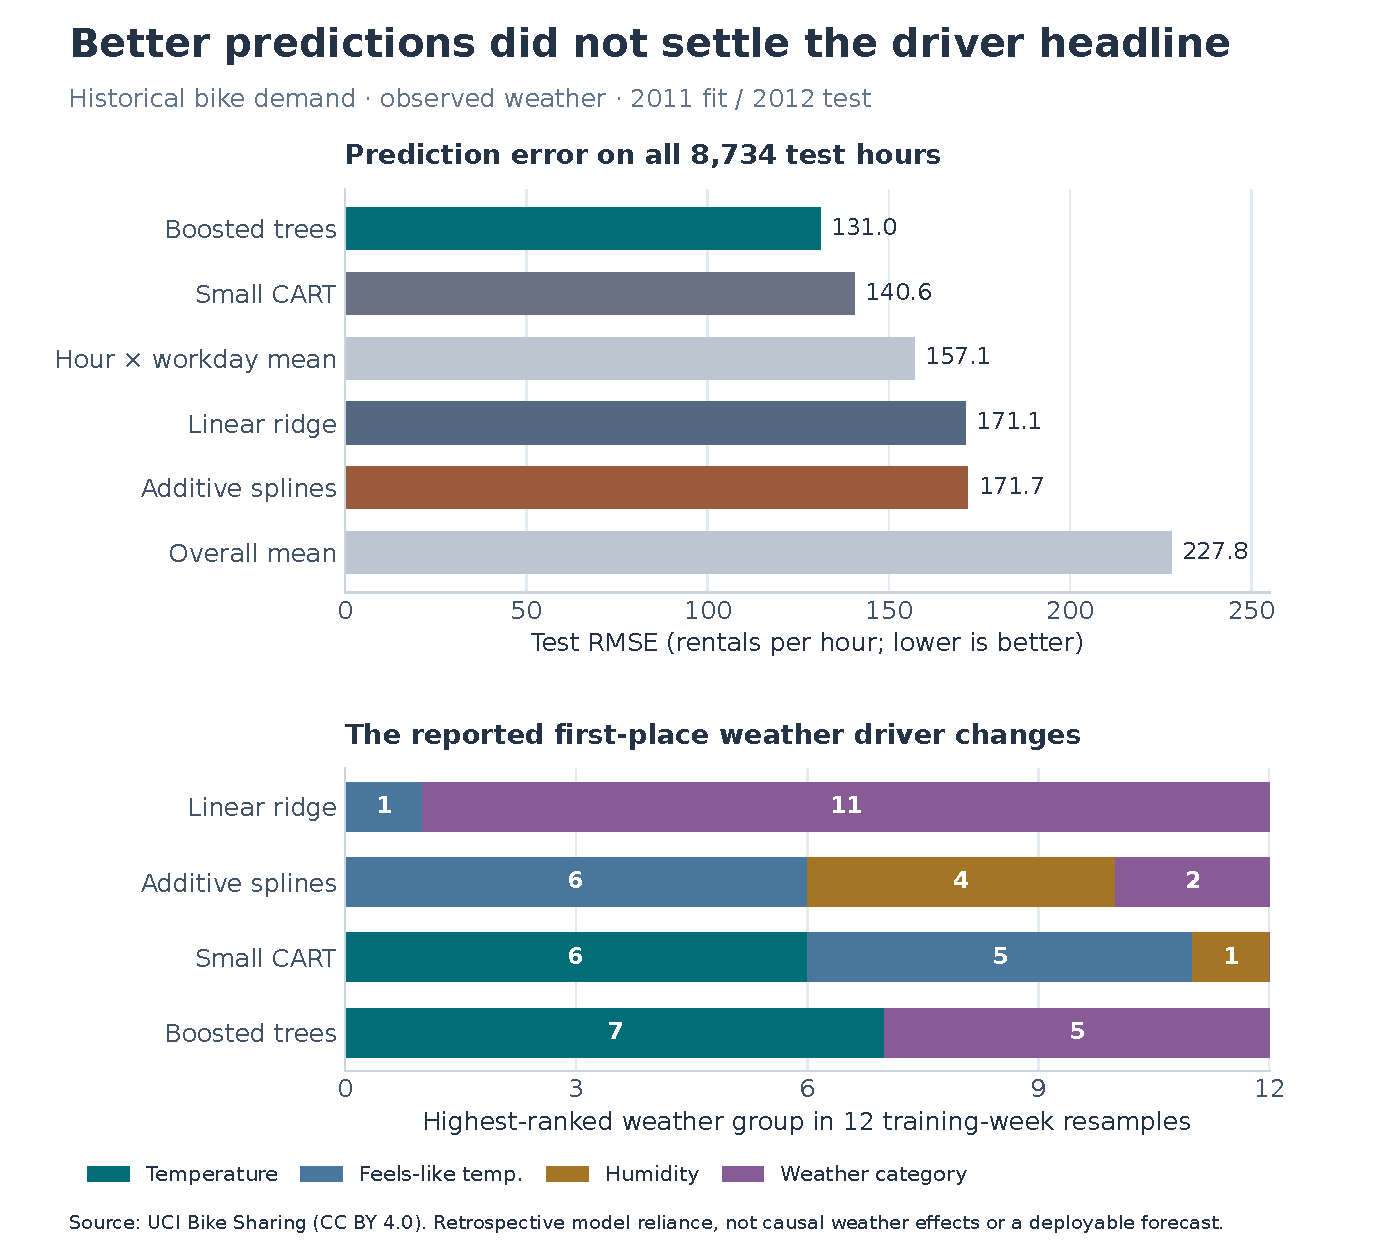
\includegraphics[width=0.98\linewidth]{images/decision-summary.pdf}
\captionof{figure}{Prediction error uses every 2012 hour. The lower panel counts the highest-ranked weather group across twelve training-week resamples per family. The full fits and resamples share the selected family-specific hyperparameters and five fixed permutation indices. These counts describe conditional training-history sensitivity, not independent deployment trials.}
\end{center}
The linear model had the most persistent individual weather leader, but its predictive error exceeded the hour-by-workday baseline. The boosted model predicted better while alternating between weather category and temperature. An explanation should therefore name the model, diagnostic and stability evidence rather than present a single driver as an established operational cause.

\clearpage
\section*{Design and protected evaluation}
\textbf{Source and population.} The original UCI Bike Sharing hourly file contains 17,379 aggregate observations from Capital Bikeshare in 2011--2012 [1]. The landing page lists 17,389; the discrepancy is retained. There are 165 absent hours within the source span. They remain missing hours, not manufactured zero demand. Every original CSV value, calendar code and total identity \(\mathrm{cnt}=\mathrm{casual}+\mathrm{registered}\) was independently reconciled. There are no individual rider records in this package.

\textbf{Model inputs.} Predictors are hour, weekday, month, workday, holiday, weather category and the supplied normalized temperature, feels-like temperature, humidity and wind speed. Target components and the record identifier are excluded. Calendar terms use fixed cyclic harmonics and one-hot categories. Ridge-family population means, standard deviations and additive-spline quantile knots are fitted only on the corresponding training sample. Source-provided weather normalization is retained.

\textbf{Selection.} Three forward 2011 folds fit through June, August and October and validate on the following two months. Their validation counts are 1,475, 1,460 and 1,460. Each family selects its lowest pooled validation MSE, with candidate-name tie handling. The complete grid has 24 settings and 72 fold fits: five ridge penalties per linear/additive family, six CART settings and eight boosting settings. All four families are reported; no test-year winner selects the narrative or hyperparameters.

For standardized ridge design \(Z\), the fitted objective is
\[
 \frac{1}{n}\sum_i(y_i-b-Z_i\beta)^2+\lambda\|\beta\|_2^2.
\]
The intercept is unpenalized. The selected linear and additive penalties are 0.01 and 0.1. CART selects depth 6 with minimum leaf 20. Boosting selects seven leaves, learning rate 0.1 and L2 penalty 1, with 120 fixed iterations and no early stopping. These are finite declared grids, not global generalization optima. The full protocol and every trial are retained.

\textbf{Training perturbations.} Complete Monday-start weeks from 2011 are sampled with replacement, including partial edge weeks as supplied. Twelve common draws are used for each selected family. Full training plus twelve refits yields 52 final variants. Every coefficient, spline transform or tree node is frozen in readable JSON before 2012 inference. Preprocessing is refitted within each resample; hyperparameters are not retuned.

\textbf{Explanation diagnostic.} A label-independent SHA-ordered subset selects 1,500 test hours. Five common permutations operate within month, hour and workday strata. Importance is the mean increase in clipped-prediction MSE after a group is moved. The same indices move both temperature columns for the joint diagnostic. There are 107 singleton rows that cannot move. Hour, month and workday themselves are structurally unchanged under these strata; their zero values do not establish lack of predictive relevance. Negative importance is retained.

\clearpage
\section*{Shortlist membership and first place answer different questions}
\begin{center}
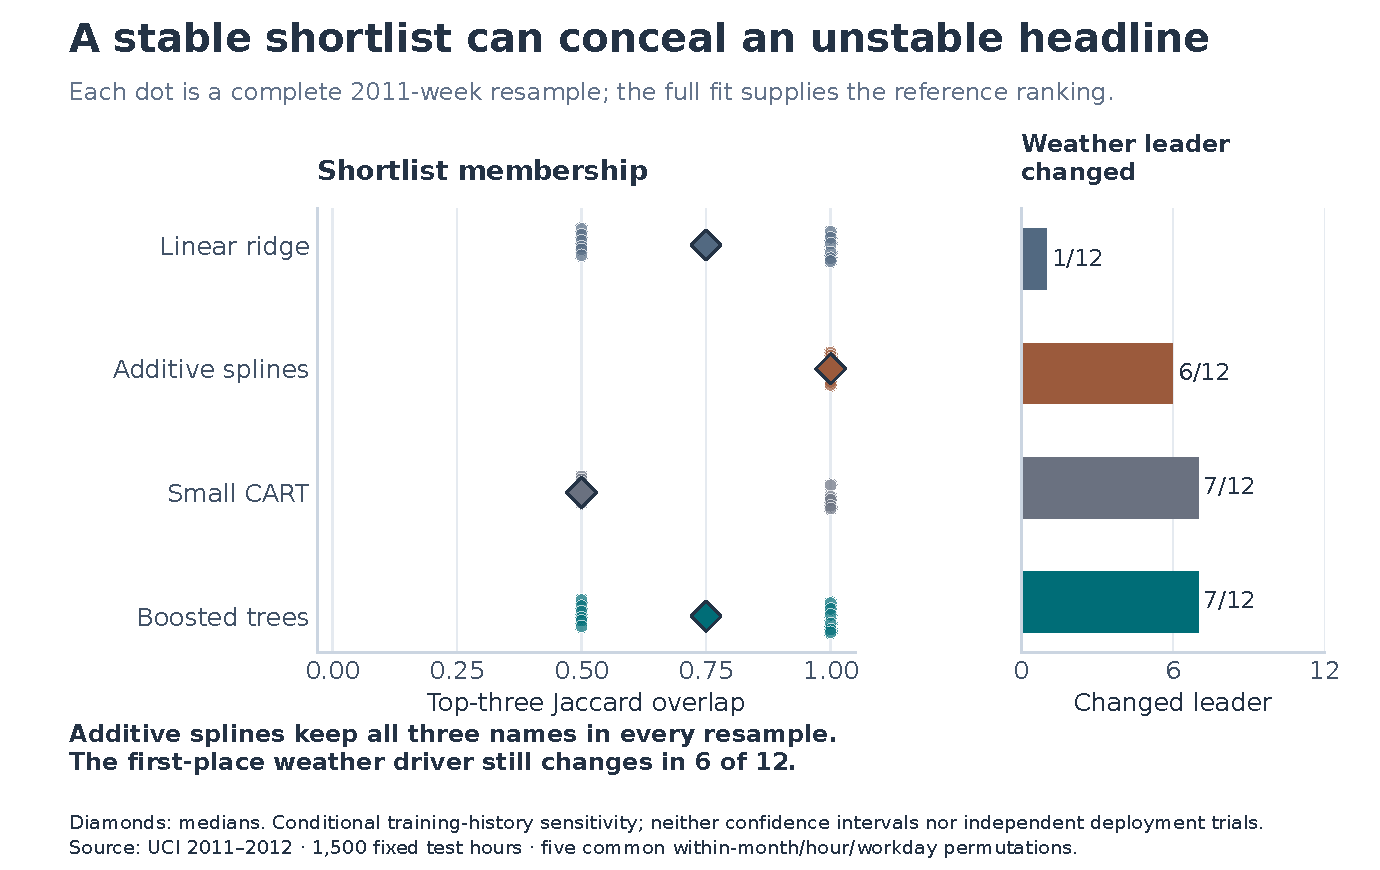
\includegraphics[width=\linewidth]{images/ranking-sensitivity.pdf}
\captionof{figure}{Top-three Jaccard overlap compares set membership with the full-training reference. The right panel separately counts changes in the first-place weather group. Dots represent all twelve resamples; diamonds are medians, not confidence limits.}
\end{center}
Additive splines had Jaccard overlap 1.0 in every resample, but the leading weather group was feels-like temperature in six, humidity in four and weather category in two. A stable group of names therefore did not make its internal order stable.

For boosting, temperature led in seven resamples and weather category in five. The full-fit reference led with weather category, so seven headlines changed. CART changed its leader seven times and reversed the temperature-versus-feels-like order seven times. The linear family reversed that pair's order five times despite weather category leading eleven of twelve refits.

Spearman correlations and all ordered ranks remain available in the public results. They are descriptive sensitivity measures with fixed alphabetical tie handling. The twelve refits share a source year and evaluation sample. Treating them as twelve independent tests, or turning their frequencies into a general confidence statement, would overstate the design.

\textbf{Reporting implication.} When a first-place claim matters, inspect first-place frequency directly. A shortlist-overlap statistic cannot substitute for that check. If the ranking changes, report the group of plausible leaders and the diagnostic conditions rather than selecting the most convenient refit.

\clearpage
\section*{The temperature grouping changes the comparison}
\begin{center}
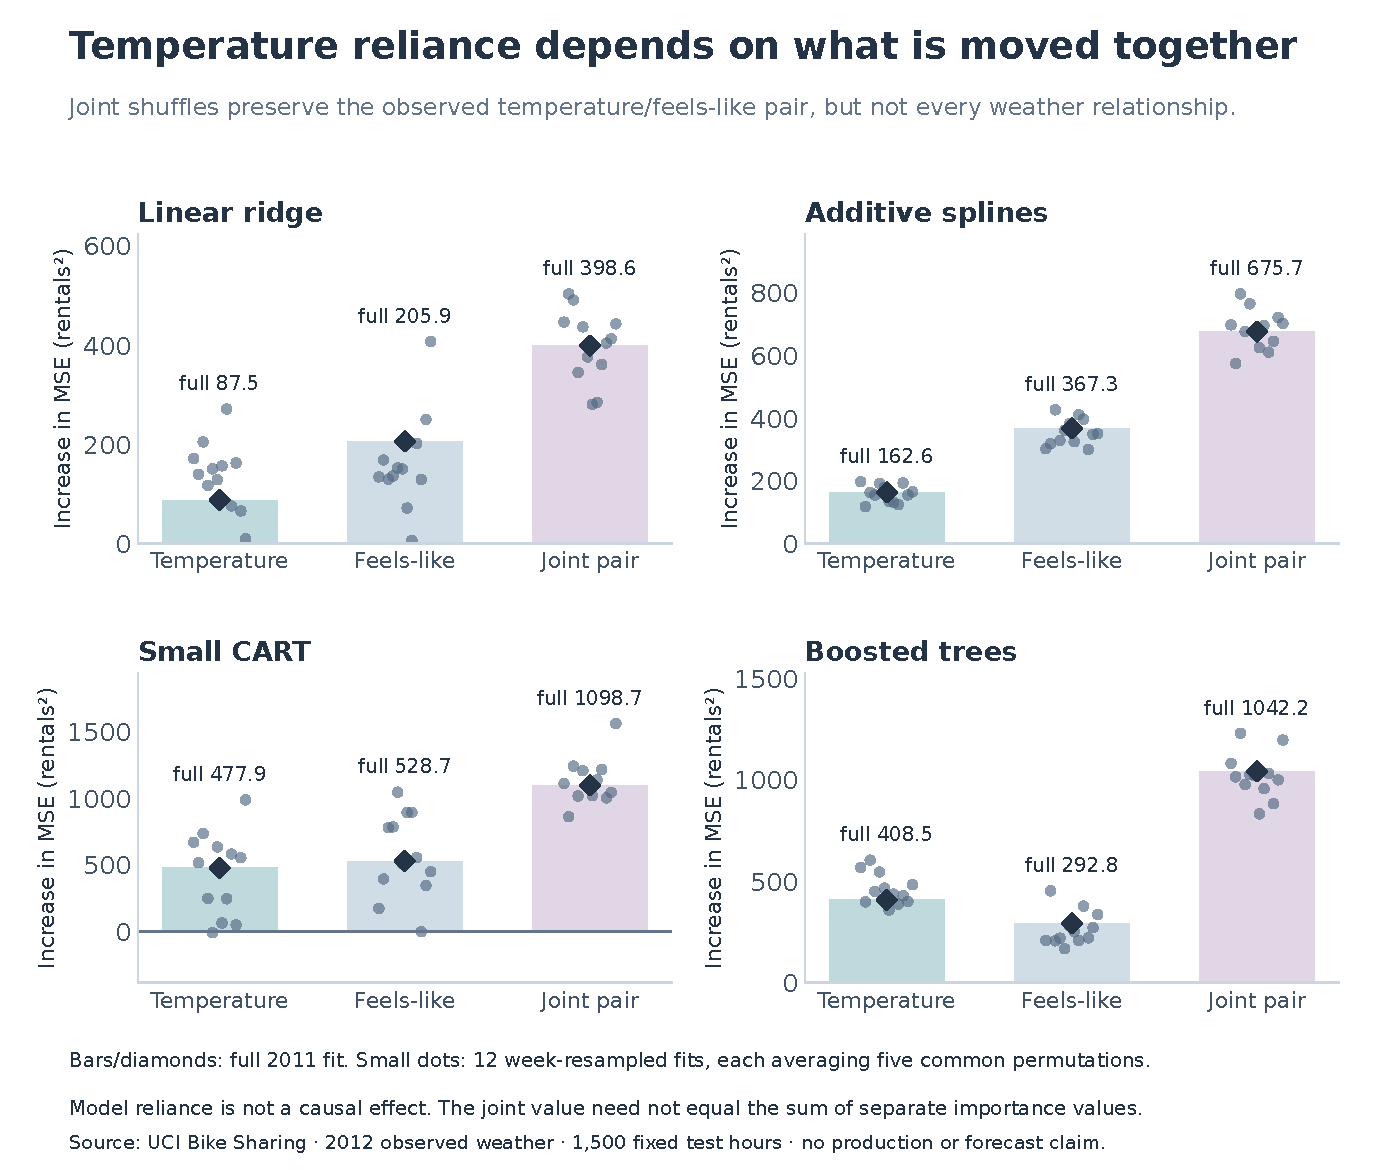
\includegraphics[width=\linewidth]{images/temperature-grouping.pdf}
\captionof{figure}{Each full-fit value and every resampled value averages five common permutations over the same 1,500 test hours. The joint diagnostic moves the observed temperature/feels-like pair together. Its value is not the sum of two individual importances. Dots show conditional refit variation, not a sampling confidence interval.}
\end{center}
Joint-temperature reliance ranked first among weather groups in all twelve resamples of the additive, CART and boosted families. In the linear family it ranked first in five and second in seven. This grouping reduced one reporting ambiguity in three families; it did not make all models or explanations agree.

The joint shuffle preserves the relationship within the pair, but can break its relationships with humidity, weather category and other covariates. Separate shuffles can also create combinations outside the observed relationship between temperature and feels-like temperature. The results measure model reliance under this operation. They do not estimate the effect of changing weather or a causal policy intervention.

\clearpage
\section*{Independent checks, limits and the next useful experiment}
\textbf{Numerical evidence.} All 105,480 validation predictions and 24 pooled candidate losses were independently recomputed. The audit verifies 124 fitted transforms and row identities, whole-week multiplicities and 56 ridge objective/gradient certificates. The maximum independent ridge gradient was \(3.27\times10^{-12}\). Positive definite penalized feature Hessians support the fixed-design convex objective; this is not a certificate of optimal predictive generalization.

All 471,636 full-test predictions and 4,290,000 permutation predictions were joined to source targets and checked for error, clipping and finite values. The independent audit reconstructs 2,860 permutation-repeat values, 572 averaged importances and 52 rank rows. Separately written scalar inference was checked at 5,720 fixed model/group/repeat cases; it was not independently rerun at every inference. Both baselines were checked at every test row.

A pre-test checker exposed a one-ulp decimal-parser difference at a spline boundary. Round-trip parsing corrected it and all fits were regenerated \emph{before} test scoring. The first failure and correction are retained. Rendering review also corrected clipped figure text. Fresh replay refits all models and checks numerical outputs at the original \(10^{-7}\) absolute and \(10^{-9}\) relative tolerances. The release requires a successful exact-revision Linux run in addition to local replay.

\textbf{Limits.} This is one historical system and one temporal holdout. Demand changes between years, the supplied weather is observed rather than forecast, and the conditioning strata deliberately restrict which comparisons can change. Twelve week resamples are a bounded sensitivity exercise. They do not prove robustness to future operations, devices, cities, policies or a different source population. Individual feature importance is not causal importance. No users, adoption, savings, revenue or production deployment are claimed.

\textbf{Next experiment.} Repeat the predeclared reporting comparison on a separate later-period system with weather-forecast vintages and an operational decision metric. Before making a headline, specify which level must be stable: predictive error, shortlist membership, first place or a scientifically defensible feature group. A prospective study should use a new protected period rather than tune against this already examined holdout.

\section*{Sources and reproducible package}
\small
[1] H. Fanaee-T (2013). \emph{Bike Sharing}. UCI Machine Learning Repository. DOI \href{https://doi.org/10.24432/C5W894}{10.24432/C5W894}. CC BY 4.0. Original archive/member hashes, source discrepancy and attribution are retained.

[2] A. Fisher, C. Rudin and F. Dominici (2019). \emph{All Models are Wrong, but Many are Useful}. JMLR 20(177), 1--81. \href{https://www.jmlr.org/papers/v20/18-760.html}{Primary article}. Model class reliance motivates examining more than one fitted model; this study does not reproduce its bounds or MCR estimator.

[3] scikit-learn 1.7 documentation. \emph{Permutation Importance with Multicollinear or Correlated Features}. \href{https://scikit-learn.org/1.7/auto_examples/inspection/plot_permutation_importance_multicollinear.html}{Official worked example}. The analysis uses pinned scikit-learn 1.7.0.

Code, eligible aggregate data, full trials, prediction exports, checks and figures:
\href{https://github.com/S3R3Bii/demand-explanation-stability}{S3R3Bii/demand-explanation-stability}. This research manuscript is shared on GitHub and has not been peer reviewed. Source papers remain outside GitHub; formal publication submission is a separate activity.
\end{document}
